% -----
% COMP 4670 Exam preparation
% Jimmy Lin
% -----
% -
\documentclass[11pt,a4paper]{article}
% package used
%{{{
\usepackage{geometry,amsthm,amsmath,graphicx}
\usepackage[colorlinks,
            linkcolor=blue,
            anchorcolor=red,
            citecolor=green
            ]{hyperref}
%}}}
\usepackage{verbatimbox}
\usepackage{tikz,multicol,amsfonts,wallpaper}
\usepackage{float}
\usetikzlibrary{automata,positioning}
% file info macros and package parameters
%{{{
\newcommand{\AUTHOR}{Jimmy Lin}
\newcommand{\UID}{u5223173}
\newcommand{\UNIVERSITY}{Australian National University}
\newcommand{\COLLEGE}{College of Engineering and Computer Science}
\newcommand{\COURSE}{COMP4670 Introduction to Machine Learning}
\newcommand{\LECTURER}{Christfried Webers}
\newcommand{\TUTOR}{Wen Shao}
\newcommand{\TASK}{Exam Preparation}

\usepackage{geometry}
\usepackage{fancyheadings}
\geometry{top=18mm,bottom=18mm,left=20mm,right=20mm}
\pagestyle{fancyplain}
\lhead{\COURSE}     
\rhead{\TASK}  
\lfoot{\copyright\ \AUTHOR\ (\UID)}
\rfoot{\UNIVERSITY}
%}}}
% new command definition
%{{{
\newcommand{\htab}{\hspace*{0.63cm}}
\newcommand{\dhtab}{\hspace*{1.26cm}}
\newcommand{\dd}[2]{\mathcal{D}\{ #1 \} (#2)}
\newcommand{\ddt}[2]{\mathcal{D}^{2}\{ #1 \} (#2)}
\newcommand{\bs}[1]{\boldsymbol{#1}}
\newcommand{\pg}{\\[0.3cm]}
\newcommand{\infint}{\int_{-\infty}^{+\infty}}
\newcommand{\dinfint}{\int_{-\infty}^{+\infty}\int_{-\infty}^{+\infty}}
\newcommand{\bmu}{\boldsymbol{\mu}}
\newcommand{\bsum}{\boldsymbol{\Sigma}}
\newcommand{\xv}{\textbf{x}}
\newcommand{\xnv}{\boldsymbol{x}_{n}}
\newcommand{\bx}{\boldsymbol{x}}
\newcommand{\R}{\mathcal{R}}
\newcommand{\W}{\boldsymbol{W}}
\newcommand{\D}{\mathcal{D}}
\newcommand{\m}{\boldsymbol{m}}
\newcommand{\V}{\mathcal{V}}
\newcommand{\N}{\mathcal{N}}
\newcommand{\BOLD}[1]{\textbf{#1}}
%}}}
%
\newcommand{\half}{\frac{1}{2}}
\DeclareMathOperator*{\argmin}{arg\,min}
\DeclareMathOperator*{\argmax}{arg\,max}
% - 
\begin{document}
21. What is the singular value decomposition of a matrix $A$. 

    Singular value decomposition of matrix $A$ is to decompose $A$ to be a product of tranpose of one orthogonal matrix $U$, one diagonal matrix $\Sigma$ whose diagonal entry is singular value of $A$ and another othogonal matrix $V$. 
    $$
     A = U^T \Sigma V
    $$

22. Calculate the gradient of the following function  
    $$
    f(X) = tr\{ X^T C X\}
    $$

    Solutions starting from definition of derivative: (Refer to Notes)
\begin{align}
    & \hspace{0.4cm} \lim_{n \rightarrow 0} \frac{ f(X + n\xi) - f (X) }{n} \\
    &= \lim_{n \rightarrow 0}  \frac{tr\{ (X + n\xi)^T C (X + n\xi)\} -  tr\{ X^T C X\}}{n} \\
    &= \lim_{n \rightarrow 0} \frac{ tr\{ (X + n\xi)^T C (X + n\xi) - X^T C X\}}{n}  \\
    &= \lim_{n \rightarrow 0}  \frac{ tr\{ X^T CX + nX^TC\xi + n\xi^T CX + n^2\xi^TC\xi- X^T C X\}}{n}  \\
    &= \lim_{n \rightarrow 0} \frac{ tr\{ nX^TC\xi + n\xi^T CX + n^2\xi^TC\xi \}}{n}  \\
    &= \lim_{n \rightarrow 0}  tr\{ \frac{ nX^TC\xi + n\xi^T CX + n^2 \xi^T C \xi}{n} \} \\
    &= \lim_{n \rightarrow 0}  tr\{ X^TC\xi + \xi^T CX + n \xi^T C \xi \} \\
    &=  tr\{ X^TC\xi + \xi^T CX  \} \\
    &=  tr\{ X^TC\xi + X^TC^T \xi  \} \\
    &=  tr\{ X^T(C + C^T)\xi  \} 
\end{align}

23. Explain the difference of frequentist's approach and Bayesian approach. (Refer to Textook P23)

    Aspects: \BOLD{objective, sequential learning, compromise}    

    Frequetist's approach is to use maixmum likelihood estimation to do point estimation of parameter $w$. Does not require preknowledge but need a large amount of data. The sequential learning is based on the sequential update formula
    $$
    w^{(\tau+1)} = w^{(\tau)} - \xi \bigtriangledown E(w)
    $$

    Whereas the bayesian approach is to derive a probability distribution over the parameter based on the Bayes Theorem. This approach does not necesarily require a large amount of data if the prior knowledge is provided. And it is inherently a good framework for sequential learning. The posterior in current iteration works as the prior in the next iteration. 
    $$
    p(w^{(\tau+1)}|t) = \frac{p(t|w^{(\tau)})p(w^{(\tau)})}{p(t)}
    $$

    According to the Bayes Theorem, there is a \BOLD{compromise} between the observation of dataset and the preknowledge. If the amount of data is very large or preknowledge (prior) provides no disparity for various classes, the preknowledge can be ignored. However, when the data is scarce, the preknowledge plays an important role.

    24. What is $S$-fold cross validation? Why we use it? (Refer to P32-33)
    
    Cross validation is Model Selection algorithm, sometimes used for determining the parameters. Randomly group all labeled data into $S$ sets, and for each model run experiment for $S$ times. At each experiment leave one set as testing set and others as training set. Extreme: leave-one-out cross validation, S = N, each set contains only one piece of labeled data.

    Reason: 
    \begin{itemize}
    \item To assess a model, performance on training set is not sufficient since it cannot be generalised to all data set.
    \item When data is scarce, and in order to assess models appropriately, we wish to use as much of the available data as possible for training.

    Drawbacks:
    \begin{itemize}
    \item The number of training runs that must be performed is increased by a factor of S, and this can prove problematic for models whose training is computationally expensive.
    \item Exploring combinations of settings for such parameters could require a number of training runs that is exponential in the number of parameters.
    \end{itemize}
\end{itemize}


25. Derive a least squre solution for linear regression model (with regularisation).
    
    The error function for least square error with regularisation:
    \begin{align}
        E(w) &= \half \sum_{n=1}^{N} (y(x_n) - t_n)^2 + \half w^T w \\
             &= \half ( w^T )
    \end{align}

    $$
    w = (\lambda I - \Phi^T \Phi)^{-1} \Phi t
    $$

    26. What is stochastic gradient descent? How to apply it to linear regression problem specifically with the sum-of-squares error function? (Refer to Textbook P144)

    Stochastic gradient descent is one optimisation algorithm, which consider only the error of one piece of observed data at each iteration of training. That is where it is different from the batch gradient descent, which takes the averaged errors of all the observed data in one training iteration.
    $$ \bs{w}^{(\tau+1)} = \bs{w}^{(\tau)} - \xi \bigtriangledown E(\bs{w}) $$

    In sum-of-square function, we have error function for one observed data as follows,
    $$ E(\bs{w}) = ( \bs{w}^T \Phi(x_n) - t_n)^2 $$
    
    whose gradient is 
    $$ \bigtriangledown E(\bs{w}) = (\bs{w}^T \Phi(x_n) - t_n) \Phi(x_n)$$
    
    Take this gradient of error function back, we have
    $$ \bs{w}^{(\tau+1)} = \bs{w}^{(\tau)} - \xi (\bs{w}^T \Phi(x_n) - t_n) \Phi(x_n) $$

27. What is the bias-variance decomposition? Demonstrate the bias-variance trade-off where the error is measured by the mean squared error. What you can deduce from the result? (Refer to Textbook P149)
    
Bias-variance trade-off is a frequentist viewpoint of the model complexity issue: \textbf{expected squared error} $\{ y(\bs{x} ; \mathcal{D}) - h(\bs{x}) \}^2$ can be decomposed as summation of squared bias and the variance.

\begin{figure}[H] \centering
    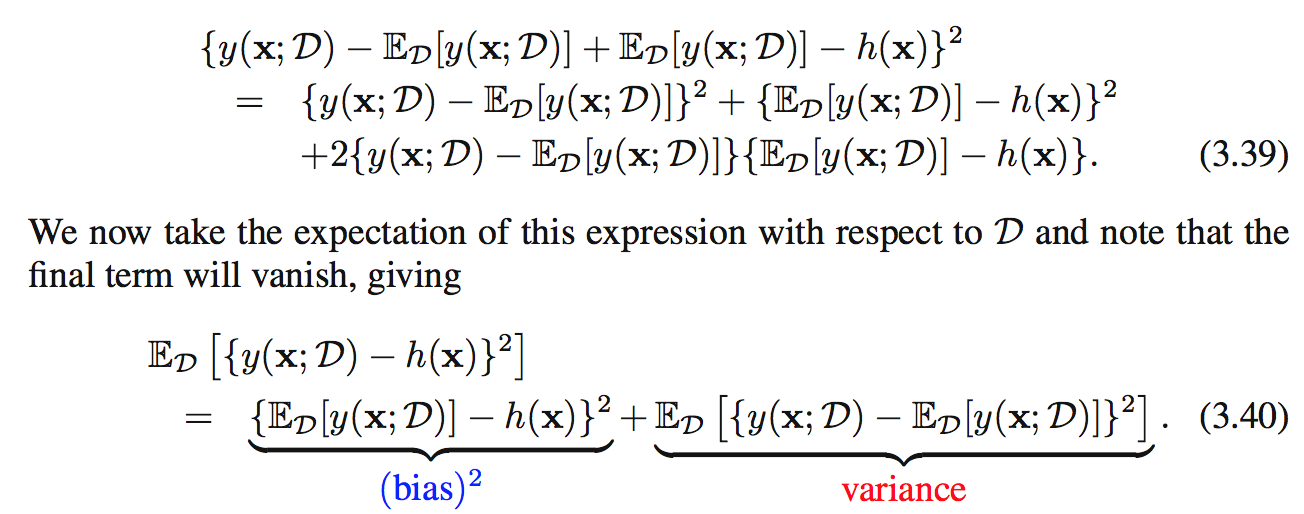
\includegraphics[width=5.5in,height=2in]{./figure/BVtradeoff.png}
    \caption{Sampling from Standard Distributions.}
\end{figure}

Deduced Condlusion: 

\begin{itemize}
    \item There is a trade-off between bias and variance, with very flexible models having low bias and high variance, and relatively rigid models having high bias and low variance.
    \item The model with the optimal predictive capability is the one that leads to the best balance between bias and variance. 
\end{itemize}

28. What is a conjugate prior? Why we normally use conjugate prior? What is the conjugate prior for Gaussian distribution? (Refer to P117)

A prior is conjugate to the likilihood function, if the posterior distribution derived from the Bayes Theorem shares the same form (perhaps with different parameters) with prior distribution. 

    Use conjugate prior to simplify the Bayesian treatment of sequential learning process, in the sense that we have the same update formula at all iterations. 

    Conjugate prior of gaussian distribution is gaussian distribution.

29. What are the limitations of linear basis function models? (Refer to Textbook P173)

    The basis functions are fixed before the data is observed. The chosen basis function may not adapt to the target function. And thus, the lower bound of the error may be quite large.

    The number of basis functions needs to grow exponentially, with the dimensionality $D$ of the input space. 

30. What is the curse of dimensionality? Why it can be a problem? (Refer to Textbook P36)

The severe difficulty that can arise in spaces of many dimensions is sometimes called the curse of dimensionality. 
Not all intuitions or even techniques developed in spaces of low dimensionality will generalize to spaces of many dimensions.
    

\BOLD{why it can be a problem?}: the number of parameter in vector $w$ we need to deal with is increased exponentially. 

By the way, in rejection sampling, there is another curse of dimensionality: the probability of rejection increases exponentially with regard to the dimensionality of the sampled space.

31. What are the three models for decision problems? How they are different?
    
    Linear Discriminant. Non-probalistic model. Use discriminant function, directly map the input pattern $x$ into class decision. (e.g. FDA, Perceptron algorithm.)

    Discrminative Model. Probalistic model which directly model the posterior distribution $p(C_1|x)$. And make decision based on that posterior distribution. (e.g. logistic regression)

    Generative Model. Probalistic model which first model the class-conditional probability distribution $p(x|C_k)$ and prior $p(C_k)$. And finally derive the posterior distribution $p(C_k|x)$ based on Bayes theorem. (e.g. naive bayes for discrete input with conditional independence assumption.)
    
    Generally, the generative model is the most expensive model because of the large number of parameter in class-conditional distribution $p(x| C_k)$ to be fitted. 

    32. What are the deficiencies of the least squares approach in linear classification? (refer Textbook P185-186)
    
    \begin{itemize}
    \item Least-squares solutions lack robustness to outliers.

    \item In some multi-class classification problems that linear decision boundaries can give excellent separation between the classes, the least squares approach will misclassify most of the points from some classes.
    \end{itemize}
    
33. What is the idea of Fisher's Linear Discriminant? Derive the fisher's linear discriminant that projects $x \in \mathbb{R}^D$ to $x \in \mathbb{R}^{D'}$ where $D > D'$.

    \BOLD{ADD something here...}

34. What is the perceptron algorithm? Describe it in detail.

    Basic idea of perceptron algorithm is to minimise the number of misclassified patterns in two-class classfication problem.

    Generalised linear model:
    $$ y(x) = f( w^T \Phi(x) ) = + 1 \ (w^T \Phi(x) > 0), -1 \ (w^T \Phi(x) < 0) $$

    Use Particular coding scheme: $+1$ for $C_1$, $-1$ for $C_2$.

    Error function is defined: 
    $$ E(w) = - \sum_{n\in \mathbb{M}} w^T \Phi(x_n) t_n $$

    Intuitively, correctly classified pattern will not contribute to the update, while misclassified pattern do. However, after the update, the correctly classified pattern in the past may turn to be wrong. 

    This algorithm guaranteed to converge, applied with stochastic gradient descent:
    $$ - w^{(\tau + 1)} \Phi(x_n) t_n = - w^{(\tau)} \Phi(x_n) t_n - (\Phi(x_n) t_n)^T \Phi(x_n) t_n < - w^{(\tau)} \Phi(x_n) t_n $$

35. What is the probalistic generative model? Describe it in detail.

    We have Naive Bayes for the generative model with discrete input. The Naive Bayes make a class conditional independence assumption: all features are independent on each other conditioned on the class.

36. What is logistic regression? Describe it in detail.

    Logistic Regression, in essence, is a discrminative model to solve the classfication problem. It directly model the posterior distribution $y_n = p(C_1 | x_n)$. Its likelihood function is 
    $$ p(t,X) = \prod_{n=1}^{N} y_{n}^{t_n} (1 - y_n) ^{1 - t_n} $$


37. What is the feature mapping in classfication problem? Why we need this feature mapping sometimes?

    Map input pattern from input space to feature space, on which the decision evaluation is based. 

    Sometimes, the patterns in input space is not linearly separable but in feature space it is linearly separable. Note that the overlapping problem cannot be solved by the mapping into feature space.

    38. What is Laplace Approximation? Why we need to do Laplace Approximation sometimes? Describe in details. (Refer to Notes)
{
    \begin{figure}[H] \centering
    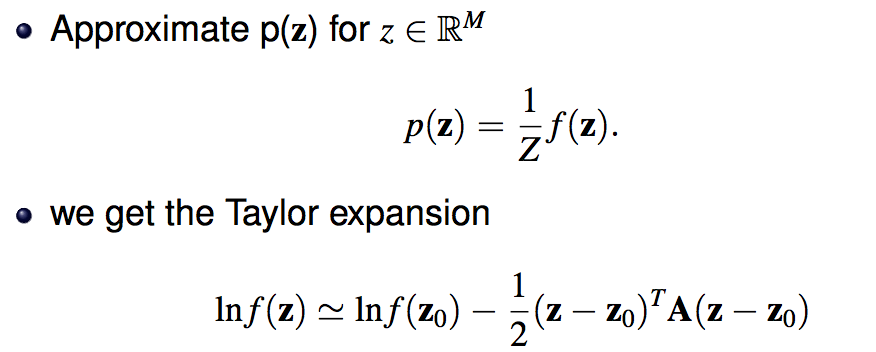
\includegraphics[width=3in,height=1.4in]{./figure/Laplace_1.png}
    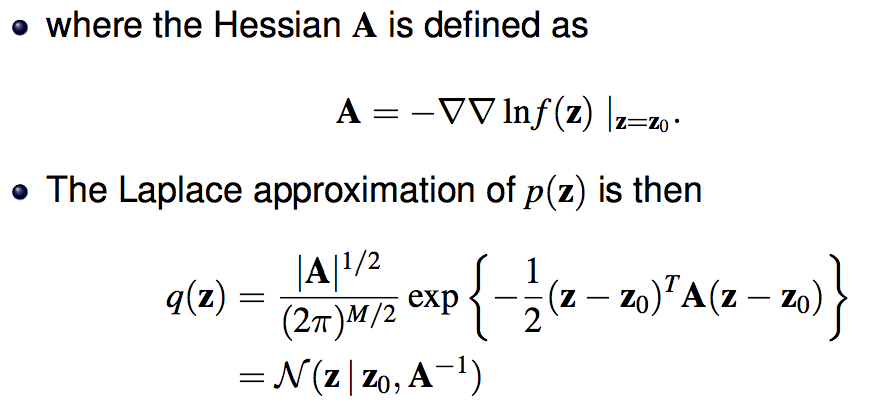
\includegraphics[width=3in,height=1.5in]{./figure/Laplace_2.png}
    \caption{Laplace Approximation in vector space.}
\end{figure}
}

39. Describe Baysian Logistic Regression in detail.

    \BOLD{ADD something here...}

    \newpage

59. Describe K-Means Clustering.

60. Describe EM algorithm for mixture of Gaussians in detail.

61. Show that Gaussian distribution belongs to exponential family.

\begin{figure}[H] \centering
    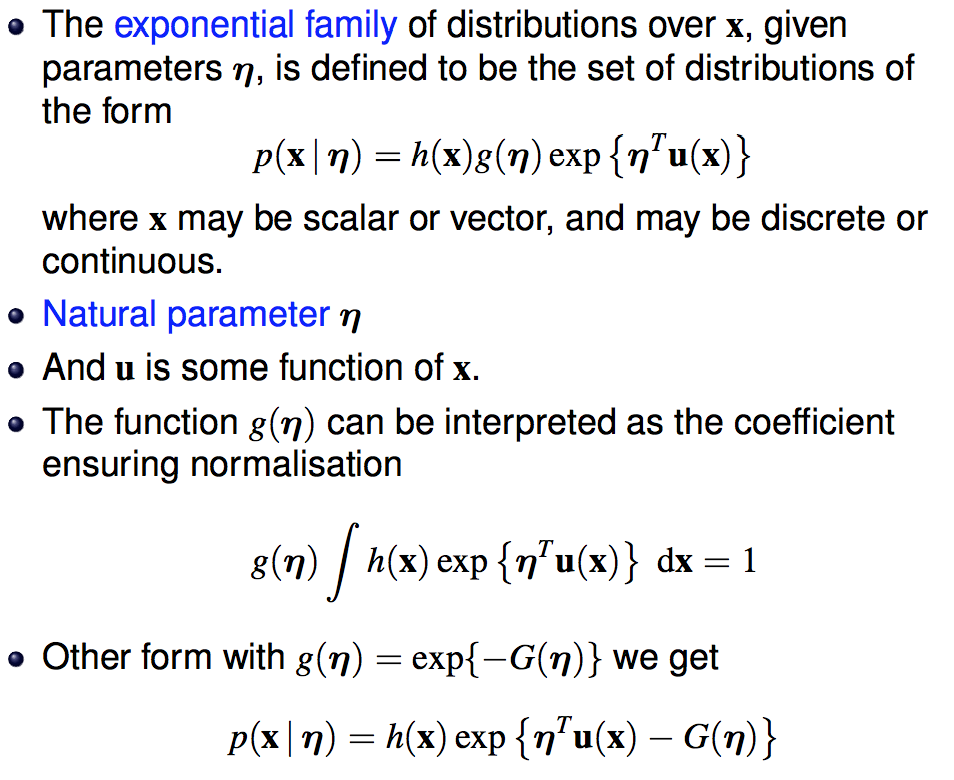
\includegraphics[width=3in,height=2.2in]{./figure/expfamily_1.png}
    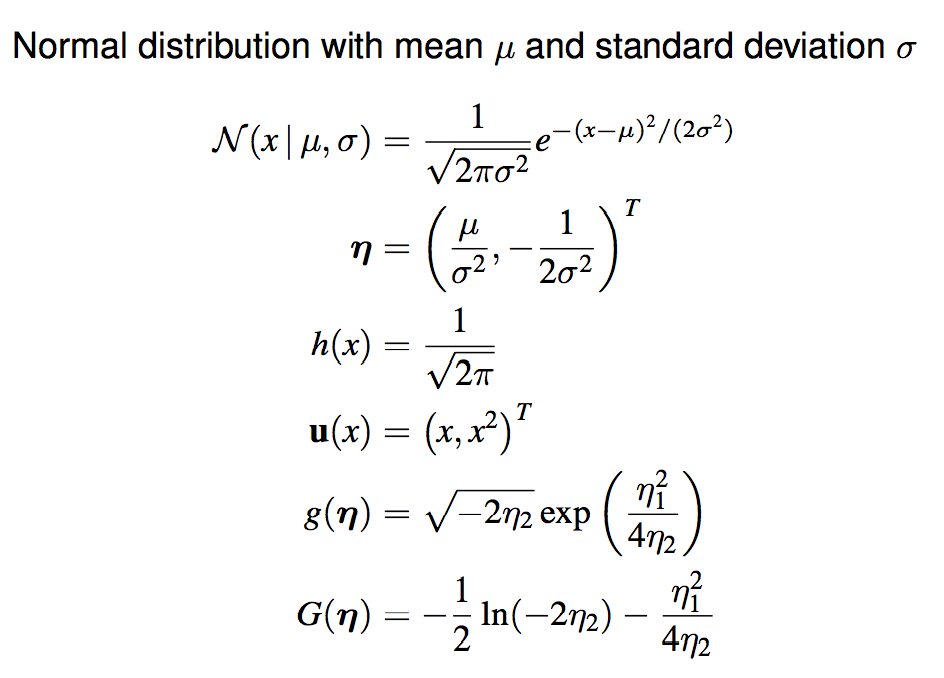
\includegraphics[width=3in,height=2.2in]{./figure/expfamily_2.png}
    \caption{Demonstrate Gaussian distribution belongs to exponential family. (eta\ $\eta$)}
\end{figure}

62. How do we sample from standard distribution? (Refer to 19\_Sampling.pdf)
\begin{figure}[H] \centering
    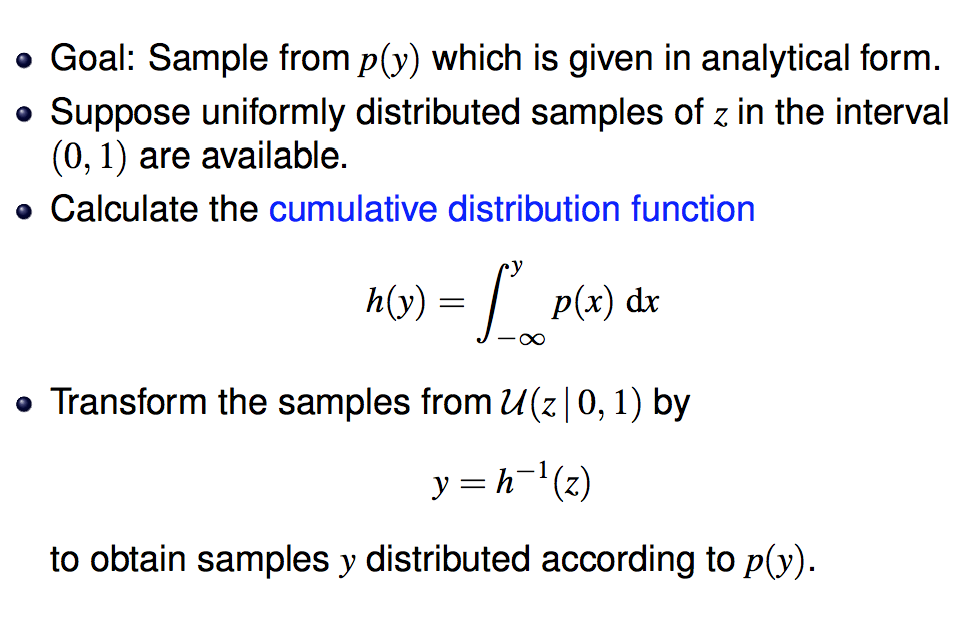
\includegraphics[width=3in,height=2.2in]{./figure/standardSampling_1.png}
    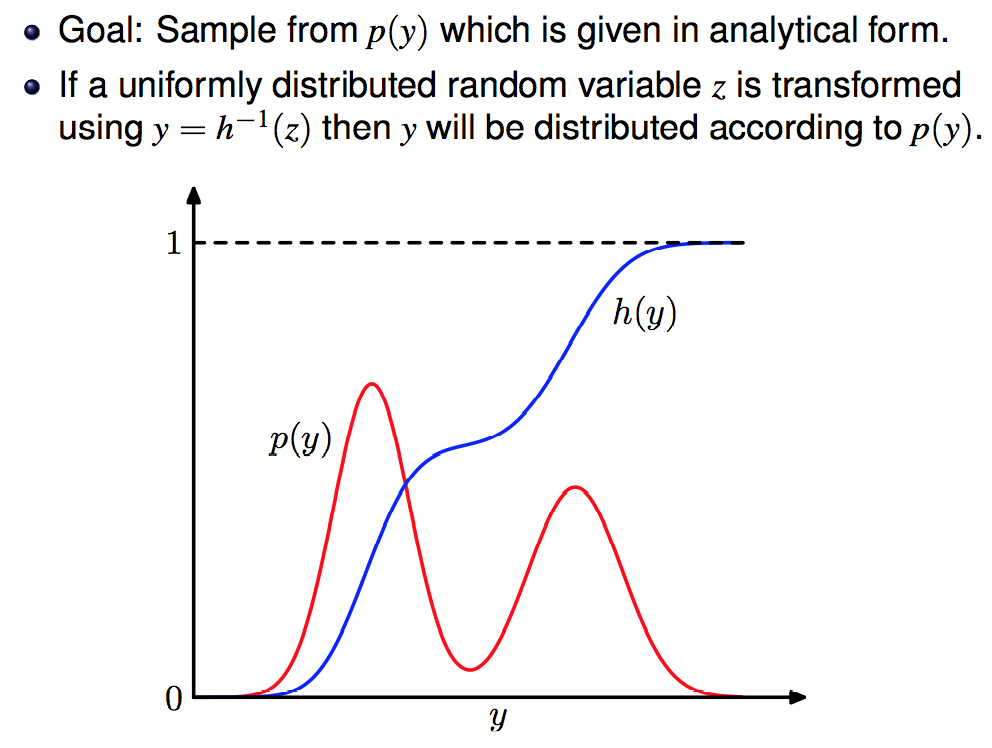
\includegraphics[width=3in,height=2.2in]{./figure/standardSampling_2.png}
    \caption{Sampling from Standard Distributions.}
\end{figure}

Last step is:
$$ p_y (y) = p_z (z) | \frac{dz}{dy}| $$

63. Describe the method you would use to sample from the following distribution:
$$ p(x=i) = \frac{1}{i} - \frac{1}{i+1},\ i = 1,2,3,4 ...$$

64. Describe rejection sampling in detail. (Refer to 19\_Sampling.pdf)
\begin{figure}[H] \centering
    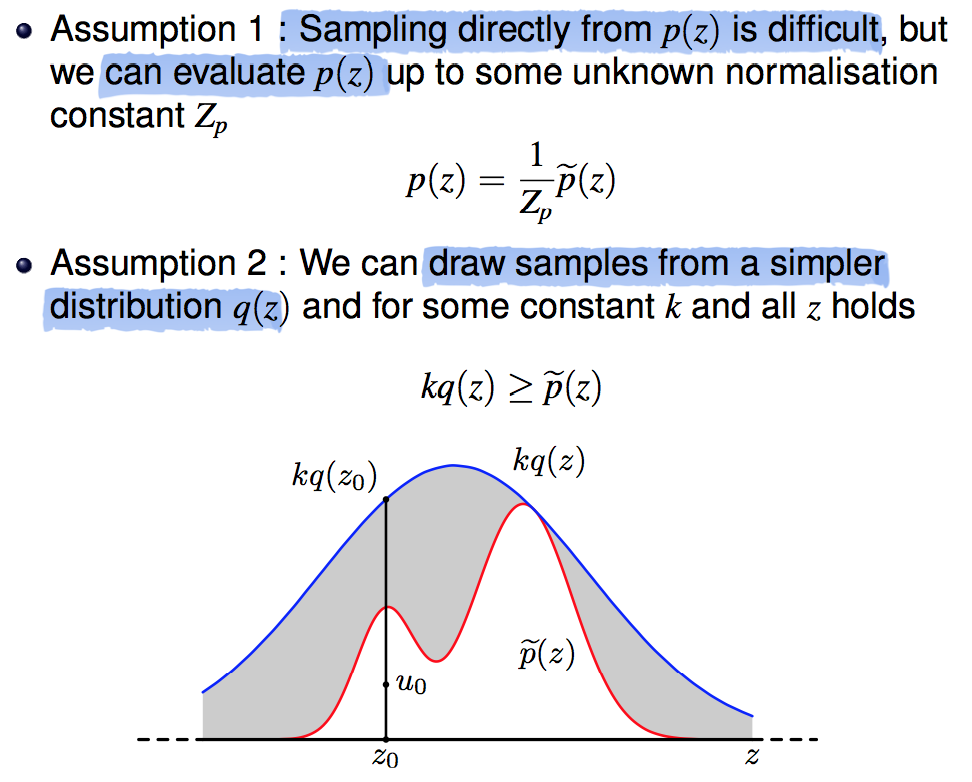
\includegraphics[width=3in,height=2.2in]{./figure/rejectSampling_1.png}
    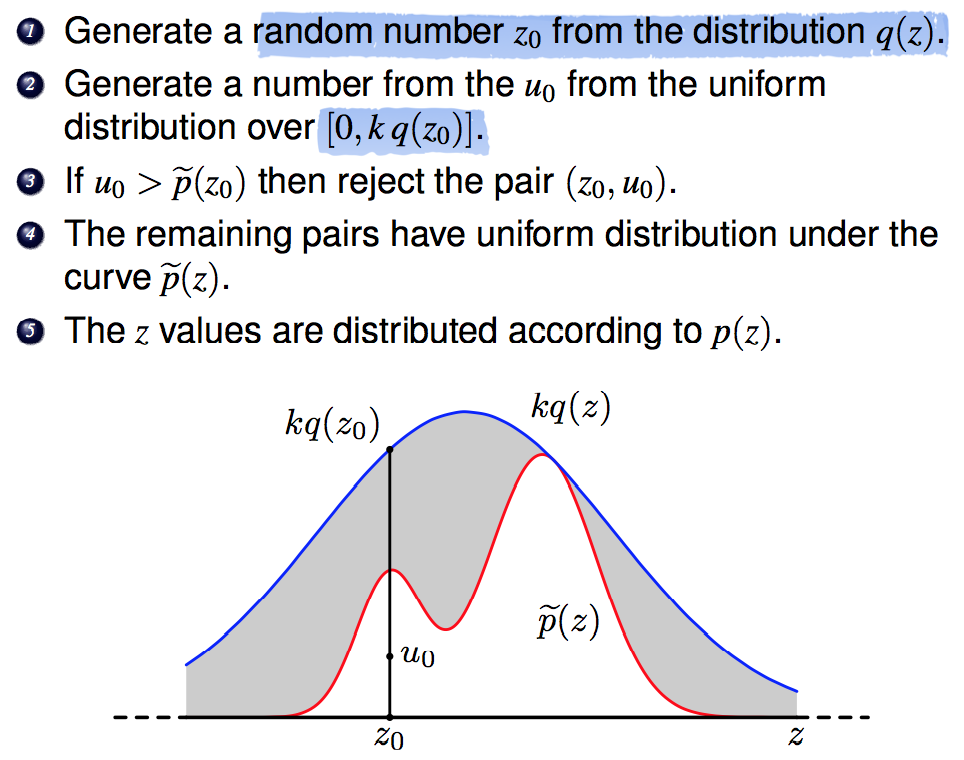
\includegraphics[width=3in,height=2.2in]{./figure/rejectSampling_2.png} \\
    \caption{Rejection Sampling Details.}
\end{figure}
\begin{figure}[H] \centering
    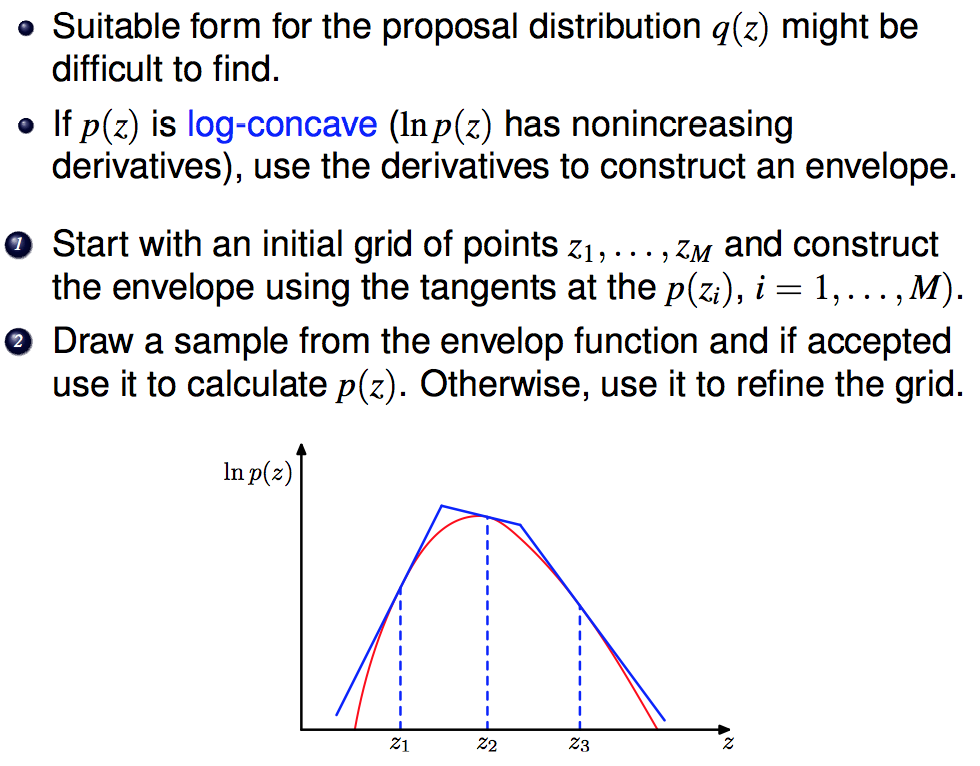
\includegraphics[width=3in,height=2.2in]{./figure/rejectSampling_3.png}
    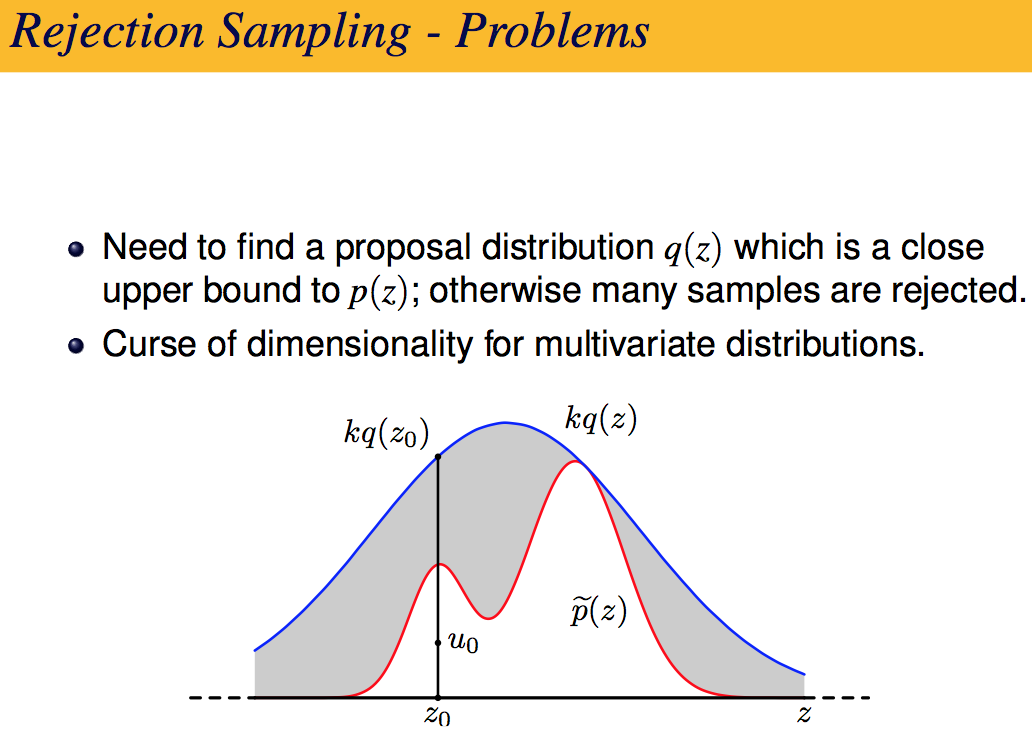
\includegraphics[width=3in,height=2.2in]{./figure/rejectSampling_4.png}
    \caption{Adaptive Rejection Sampling. Problem of rejection sampling.}
\end{figure}

65. Describe importance sampling in detail.
\begin{figure}[H] \centering
    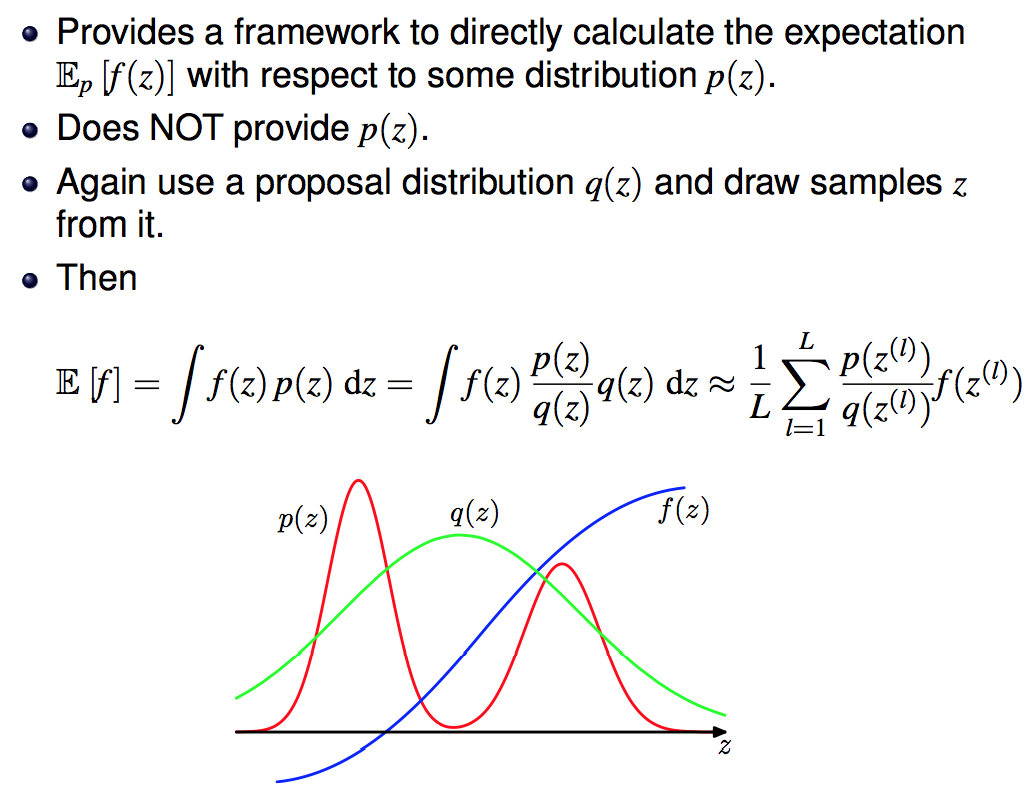
\includegraphics[width=3in,height=2.2in]{./figure/importanceSampling_1.png}
    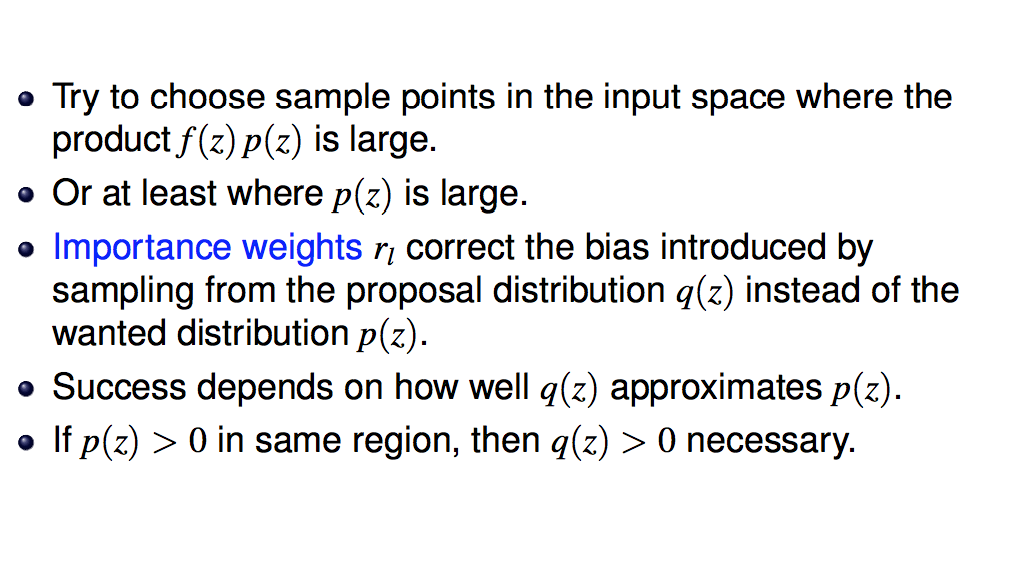
\includegraphics[width=3in,height=2.2in]{./figure/importanceSampling_2.png}
    \caption{Adaptive Rejection Sampling. Problem of rejection sampling.}
\end{figure}

66. Describe Metropolis-Hasting algorithm in detail.

67. (not sure) What is the idea behind principle component analysis?

(1) PCA is an algorithm for unsupervised learning. (differ from FDA)

(2) Functionality: Dimensionality Reduction. Project data into a subspace such that 
\begin{itemize}
    \item data objects span the most widely on the bases of projected subspace.
    \item covariance of data objects would be reduced in the least degree. info retained.
\end{itemize}

(3) Functionality: Data Decorelation. Transform the coordinate of original space and apply the scaling on each coordinate axis, such that in new coordinate system, the mean of data objects is zero and covariance matrix is identity.

68. What is a non-stationary sequential distribution? (Refer to Textbook P606)

\begin{itemize}
     \item In the stationary case, the data evolves in time, but the distribution from which it is generated remains the same.
     \item For the more complex nonstationary situation, the generative distribution itself is evolving (varying) with time. 
    \end{itemize}
Note that in this course, we just focus on stationary distribution.

69. Use a Bayesian Network to represent a second-order Markov chain. (Refer to Textbook P608)

$$ p(x_1, x_2, \cdots, x_n) = p(x_1) \ p(x_2 | x_1) \prod_{n=3}^{N} p(x_n | x_{n-1}, x_{n-2}) $$
\begin{figure}[H] \centering
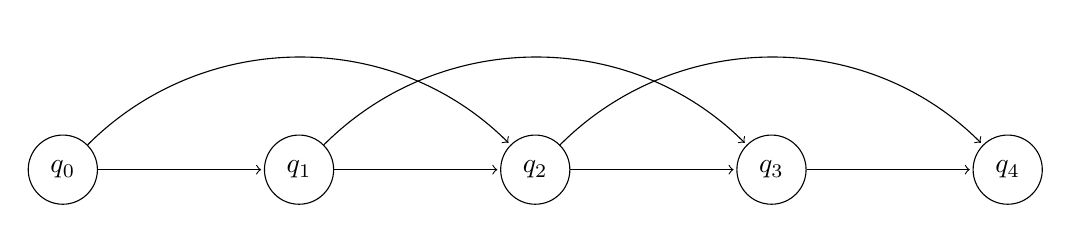
\begin{tikzpicture}[shorten >=1pt,accepting/.style={double distance=2pt},on grid,node distance=3cm,auto,bend angle=45] 
   \node[state] (s0)  {$q_0$}; 
   \node[state] (s1) [right=of s0] {$q_{1}$}; 
   \node[state] (s2) [right=of s1] {$q_{2}$}; 
   \node[state] (s3) [right=of s2] {$q_{3}$}; 
   \node[state] (s4) [right=of s3] {$q_4$};
   \path[->] (s0) edge [right] node  {} (s1);
   \path[->] (s1) edge [right] node  {} (s2);
   \path[->] (s2) edge [right] node  {} (s3);
   \path[->] (s3) edge [right] node  {} (s4);
   \path[->] (s0) edge [bend left] node  {} (s2);
   \path[->] (s1) edge [bend left] node  {} (s3);
   \path[->] (s2) edge [bend left] node  {} (s4);
\end{tikzpicture}\\[0.5cm]
\caption{Bayesian Network to represent second-order Markov Chain}
\end{figure}

70. What is the difference between principle component analysis and Fisher's discriminant? (Refer to Textbook P568)

    Similarity: Both methods can be viewed as techniques for linear dimensionality reduction.
    
    Differences:
    \begin{itemize}
        \item Essence: PCA is unsupervised learning which only considers patterns $\bs{x}_n$. FDA is supervised learning also using class-label information.
    \item Basic Idea: FDA, given the labels, maximise the between-class covariance and minimise the within-class covariance. PCA consider the maximally reserved data variance (information).
     \end{itemize}

71. Prove that independence of two random variable implies uncorrelatedness. Give counter example to show that uncorrelatedness does not imply independence. (Refer to \url{http://mathforum.org/library/drmath/view/64808.html})

    Independence: $ P (x,y) = p(x) p(y) $.  Uncorrelatedness: $ cov (x,y) = 0 $

    Proof of $independence \rightarrow uncorrelatedness$:
    \begin{align}
        Cov(X,Y) &= \infint \infint (x - E(x))(y - E(y)) p(x,y) dx dy  \\
        &= \infint \infint (x - E(x))(y - E(y))  p(x)p(y) dx dy \\
        &= \big( \infint (x - E(x)) p(x) dx \big) \cdot \big( \infint (y - E(y)) p(y) dy \big) \\
        &=  E(x - E(x)) \cdot E(y - E(y)) \\
        &=  0 
    \end{align}

    Counter-example: 

    Suppose $X$ is a normally-distributed random variable with zero mean.  Let Y = $X^2$.  Clearly X and Y are not independent.
    However, The covariance of X and Y is
    $$ Cov(X,Y) = E(XY) - E(X)E(Y) = E(X^3) - 0*E(Y) = E(X^3)  = 0 $$

72. Assuming K different states for each variable $x$, how many parameters does M-order Markov chain have? (Refer to textbook P609)
    
$ K^M (K - 1)$. $K$ is number of discrete assignments. $K^M$ is the number of possible composite assignments of $M$ conditioned variables. $K-1$ is for each possible assignment, the number of free parameters (given the normalisation property).

 Because this grows exponentially with M , it will often render this approach impractical for larger values of order $M$.

 Note that we only talk about stationary case (each factor shares the same probability distribution).

 73. What is a homogeneous hidden Markov Model? (Refer to textbook P612)
    $$ p(x_1, \cdots, x_n, z_1, \cdots, z_n) = p(z_1) \cdot \prod_{n=1}^{N} p(z_n | z_{n-1}) \cdot \prod_{n=1}^{N} p(x_n | z_n) $$

    Homogeneousness in hidden markov model means that
    \begin{itemize}
        \item all the transition probabilities $p(z_n | z_{n-1})$ share the same parameters $A$. ($A$ is transition matrix from 1-of-k coding)
        \item all of the emission distributions $p(x_n | z_n)$ share the same parameters $\Phi$.
        \end{itemize}

    The probability distribution of latent variable is \BOLD{invariant or stationary} if the \BOLD{Detailed balance} is satisfied. (also called \BOLD{reversible}.)
    $$ p^{*}(z) T(z,z') = p^{*}(z')T(z', z) $$

74. Describe Viterbi algorithm in detail.
    to find the most probable sequence of hidden states for a given observation sequence. this can be solved efficiently using the max-sum algorithm
    the problem of finding the most probable sequence of latent states is not the same as that of finding the set of states that are individually the most probable.
    max-sum algorithm works with log probabilities and so there is no need to use re-scaled variables
    The Viterbi algorithm searches this space of paths efficiently to find the most probable path with a computational cost that grows only linearly with the length of the chain.

75. What are the motivations for combining models? (refer to Lecture Notes)
    \begin{itemize}
    \item Motivation: Coming up with a very precise prediction rule can be very hard. It may be easier to come up with a number of not so precise prediction rules.
    \item Basic Idea: Combine models with different rules to make better prediction.
        \end{itemize}
\textcolor{blue}{\rule{\textwidth}{1mm}}

76. Explain differene between model combination and bayesian averaging.

Model Combination: different data points within the data set can potentially be generated from different values of the latent variable z and hence by different components.
$$ p(\bs{x}) = \sum_{\bs{z}} p(\bs{x},\bs{z}) $$

Bayesian Averaging: every hypothesis is responsible for generating the whole set of data.
$$ p(\bs{X}) = \sum_{h} p(\bs{X} | h) p(h) $$

\newpage
\BOLD{Distinction Questions}: 

1. explain how neural network function? including the back propagation with formula.

2. compare online processing  

3. explain graph separation in markov random field.

4. explain gaussian mixture model. How do you do inference in gaussian mixture model.

5. explain how hidden markov model is an extended markov chain.

we wish to build a model for sequences that is not limited by the Markov assumption to any order and yet that can be specified using a limited number of free parameters.
We can achieve this by introducing additional latent variables to permit a rich class of models to be constructed.

\BOLD{HD Questions}:

6. explain three models for classification.

7. What is bias-variance trade-off.

8. what is Fisher discriminant analysis.

\BOLD{HHD Questions}:

9. Explain how variational optimisation can be used in finding approximation for posterior distribution.

\end{document}

